\documentclass[conference]{IEEEtran}
\usepackage{graphicx}
\usepackage{float}  % Needed for the 'H' specifier

% Ensure single spacing
\linespread{1.25}
\title{%
  Pokémon Rank Classifier \\
  \large ECS 171 Fall 2023 \\
    Group 8}
    
\author{
\IEEEauthorblockN{Alexander D'souza}
\and
\IEEEauthorblockN{Catherine Chen}
\and
\IEEEauthorblockN{Shane Kim}
\and
\IEEEauthorblockN{Varun Wadhwa}
}

% \date{\textbf{Github Repository: }https://github.com/AlexanderDsouza/ECS171GroupProject}

\begin{document}
    \maketitle
\section{Introduction}
Pokémon is one of the most popular franchises in the world, with various console games, mobile apps, and a very passionate trading card collecting community. There are over 8 million daily Pokémon Go players, over 480 million lifetime console game sales, and over 3.7 billion Pokémon cards sold in the 2020-2021 fiscal year. The biggest Pokémon tournament is the Pokémon World Championship with over 110,000 dollars in prize money, so every advantage a player can get is extremely valuable. A big advantage that players can get is being able to categorize Pokémon with regards to their strength level. There are a couple of reasons this is advantageous:


\subsection{Accurately measuring the overall strength of a team}
\begin{itemize}
\item Tournaments ban certain Pokémon that are considered too “strong” so a player's team will be made up of Pokémon from various strength levels. Therefore, to know the overall strength of a player's roster, knowing the individual strength of each Pokémon is crucial. Being able to accurately measure the overall strength of a team also allows a player to know how their roster stacks up against an opposing player's roster. 
\begin{itemize}
    \item This allows players to strategically choose Pokémon to fill their team as well as determine movesets
\end{itemize}  
\end{itemize}
\subsection{Efficient Training}
\begin{itemize}
    \item A Pokémon's base stats can be improved via a concept known as Effort Values by battling other Pokémon. Therefore knowing the strength level of an individual Pokémon can allow a player to determine which Pokémon need to be trained more.
\end{itemize}


\subsection{Predictions}\label{AA}
\begin{itemize}
    \item Knowing the objective strength level of a Pokémon, allows a player to predict what moves their opponent will make against theirs. If a Pokémon is “strong” , moves that lower its attack or defense stats may be used. If a Pokémon is weak, one shot moves may be preferred.
\end{itemize}

The current issue around categorizing Pokémon is that there is no single statistic that determines if a Pokémon is strong. For example, one Pokémon may have strong attack statistics and one Pokémon may have strong defense statistics so in order to determine which Pokémon is stronger, various statistics must be considered. Even if an individual is able to manually categorize all 1021 Pokémon using their own methodology, new Pokémon are frequently released, so manually evaluating each Pokémon and comparing them to create strength tiers is not feasible. Machine learning poses an elegant solution to this issue, as being able to produce strength level predictions for new Pokémon based on previous 


\section{Literature review}
There have been previous attempts to predict or categorize attributes of Pokémon such as strength.

For example, Breddan\footnote{(Breddan, 2021)} attempted to use machine learning to answer the following questions: How are different statistics such as type, hp, attack, defense, special attack, special defense, speed, and total strength (defined as sum of statistics)  related? Can distinct groups of Pokémon be made based on these statistics to help a player diversify their team? Can predictions of one statistic of a Pokémon be made based on other statistics in order to predict a new Pokémons stats based on educated guesses? The relevance of the last question also relates to our project goal as our model can be used to predict new generation Pokémon strength based on their statistics. Breddan used both k-means classification and Random Forest Regression to answer these questions. When performing k-means classification with speed and HP as data, Breddan was able to create 5 distinct groups of Pokémon. When performing Random Forest Regression, Breddan attempted to predict total strength. The findings concluded that total strength was best predicted with a maximum tree depth of 11 and was predicted with an accuracy of 95\%, as demonstreated in Fig. 1.

\begin{figure*}
  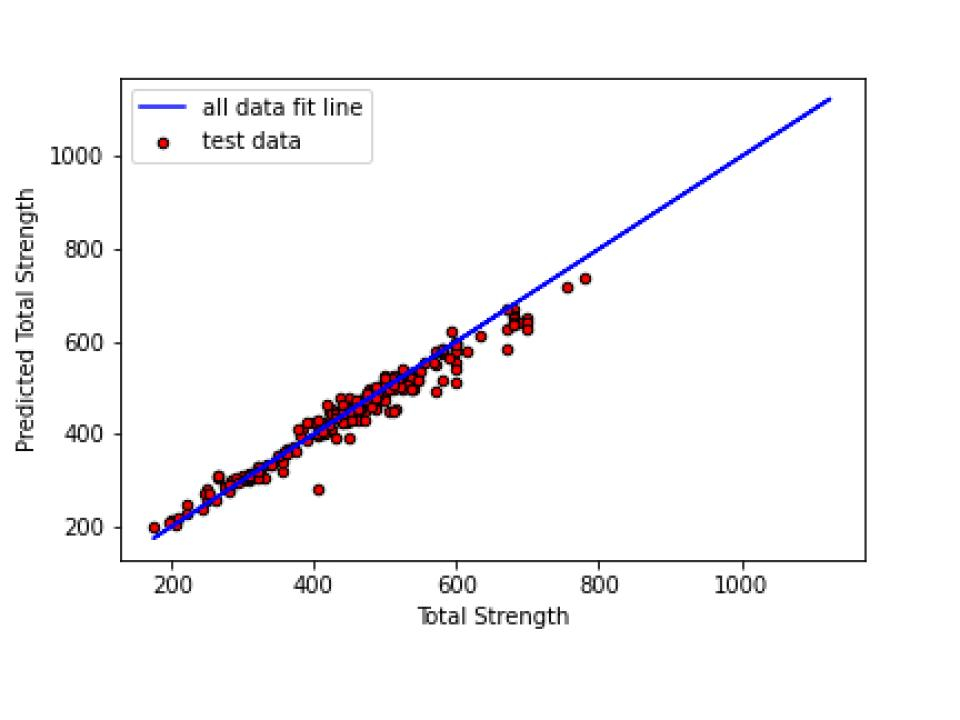
\includegraphics[width=1\linewidth]{fig1.jpg}
  \caption{Random Forest Regression model prediction results for total strength in test data set (red points) plotted against true fit line (blue).}
  \label{fig:your_photo}
\end{figure*}
            
\section{Dataset Description}
  The dataset being used in this project is a csv file sourced from Kaggle\footnote{(Data of 1017 Pokemons," September 25, 2023)}, which was produced by scraping pokeapi.co using python. There are 1017 rows in the dataset and 18 columns:

\begin{itemize}
    \item \textbf{Columns:} 
    \begin{itemize}
        \item ID of the Pokémon
        \item Name
        \item Rank (strength level)
        \item Generation
        \item Evolution chain
        \item Primary type
        \item Secondary type
        \item HP
        \item Attack
        \item Defense
        \item Special attack
        \item Special defense
        \item Speed
        \item Total stats
        \item Height
        \item Weight
        \item Abilities
        \item Description in English        
    \end{itemize}
\end{itemize}

For our model we chose to only take into account numerical data for our input features and exclude primary type, secondary type, abilities, previous evolution, and abilities. We felt that including these categorical features in our model via one hot encoding would greatly increase our model's complexity and the time it would take to train it. Our target variable is Rank, which we are using as a measure of strength. Rank has 4 categories (strength levels), legendary, mythical, legendary, baby, and ordinary. We determined that baby and ordinary, and mythical and legendary are redundant labels respectively in terms of strength level, so we categorized all ‘baby' Pokémon as ‘ordinary' and ‘mythical' as ‘legendary'. 
In order to determine which type of model to use we wanted to find out if our classes were linearly separable. We did this by making a pair plot of all the attributes, demonstrated in Fig. 2. From the pair plot we determined that our data is linearly separable based on the feature ‘total', which is the sum of all the statistics. Because of this conclusion we decided to create a linear SVM model as the data appeared to be separable by a linear decision boundary.

\begin{figure*}
    \centering
    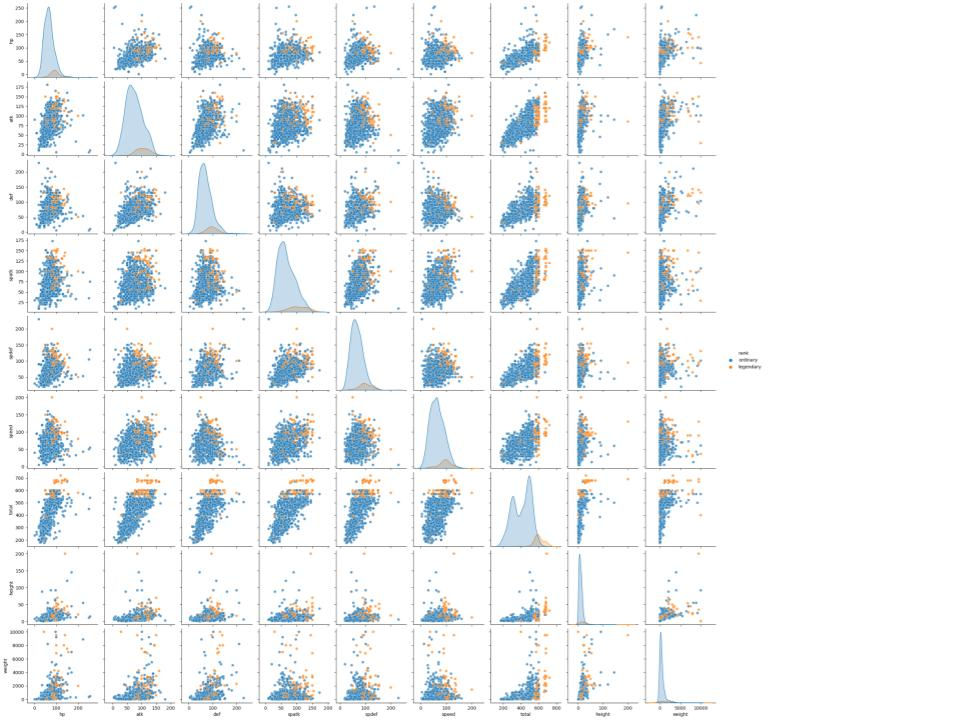
\includegraphics[width=1.3\textwidth]{Fig2.jpg} % Adjust the width as needed
    \caption{Pair Plot of the Dataset}
    \label{fig:dataset-pairplot}
\end{figure*}
We also created histograms for each feature to understand the distribution of the data. When examining the histogram for total stats, we found that the total stats for Ordinary Pokémon was bimodal and symmetric, whereas for Legendary Pokémon it was skewed to the left. This indicated that legendary Pokémon were more likely to have total stats on the higher end compared to ordinary Pokémon and further confirmed our belief that the data was linearly separable via total.

\begin{figure*}
  \centering
  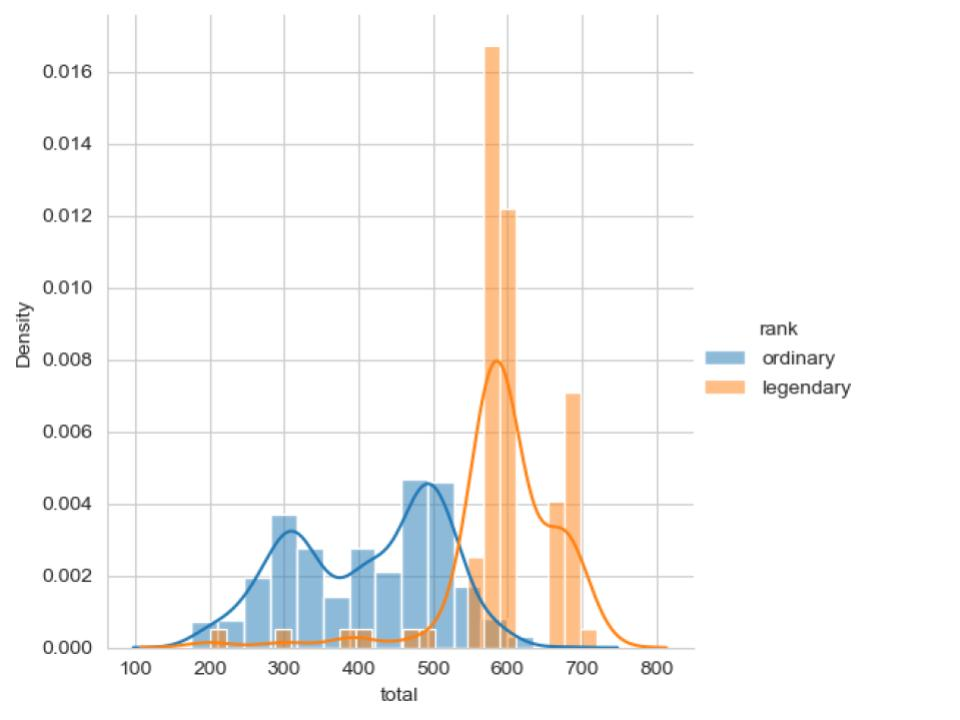
\includegraphics[width=1\linewidth]{Fig3.jpg}
  \caption{Histogram of Total Stats}
  \label{fig:your_photo}
\end{figure*}

\section{Proposed Methodology}
\subsection{Model selection}
For our Pokémon rank classifier, we opted to utilize Logistic Regression and Support Vector Machine (SVM) models due to their distinct advantages and capabilities in handling this classification task.

\subsection{Logistic Regression}
\textbf{Pros:}
\begin{itemize}
    \item Well-suited for binary classification problems like ours.
    \item Offers probabilistic interpretation of results.
    \item Generally less prone to overfitting.
\end{itemize}

\textbf{Cons:}
\begin{itemize}
    \item Assumes linear relationship between features and the log-odds of the outcome.
    \item May not perform optimally with non-linear data distributions.
\end{itemize}

\subsection{Support Vector Machine (SVM)}
\textbf{Pros:}
\begin{itemize}
    \item Effective in high-dimensional spaces.
    \item Versatile due to different kernel functions.
    \item Robust against overfitting in high-dimensional spaces.
\end{itemize}

\textbf{Cons:}
\begin{itemize}
    \item Computationally intensive with larger datasets.
    \item Choice of kernel and parameters crucial for performance.
\end{itemize}

\subsection{User Prediction Interface}

Our classifier allows users to predict whether a chosen Pokémon is legendary or not. Initially, we considered enabling users to specify the Effort Values (EVs) of the Pokémon. However, for simplicity and consistency with our test data, users can select a Pokémon, and our system will randomly distribute their EVs within allowable constraints.

\subsection{Data Augmentation}

To enhance our dataset and balance class representation, we augmented the dataset by generating additional data points. We increased the representation of 'legendary' Pokémon to ensure robustness in the training phase.

\subsection{Model Training and Evaluation}

\textbf{Data Preprocessing:} We preprocessed the data, removing unnecessary features and ensuring numerical consistency.

\textbf{Model Training:} We trained both Logistic Regression and SVM models on the augmented dataset.

\textbf{Model Evaluation:} Using train-test splitting, we evaluated the models' performance and obtained classification reports for each model.

\subsection{Model Persistence}

Upon successful training and evaluation, we persisted the SVM model as 'Pokémon\_Predictor.pkl', enabling the deployment of the trained model for future predictions.

\section{Experimental Results}
\subsection{Model Training}
Both logistic regression and SVM models were trained using a labeled dataset containing information on Pokémon attributes such as total stats, types, abilities, etc. The models were trained to predict whether a Pokémon is "legendary" or "ordinary" based on these features.

The logistic regression model was trained using gradient descent or other optimization techniques to minimize the logistic loss function and learn the optimal coefficients for the linear relationship between features and the probability of Pokémon ranks.

The SVM model, on the other hand, was trained to find the hyperplane that best separates "legendary" and "ordinary" Pokémon in the feature space. It maximizes the margin between classes while minimizing classification errors.

\subsection{SVM Model Performance}
\subsubsection{Explanation of Metrics for SVM Model}
    \begin{itemize}
        \item \textbf{Precision:} Measures the accuracy of positive predictions made by the model, indicating how accurately the SVM identifies "legendary" or "ordinary" Pokémon.
        \item \textbf{Recall:} Indicates the model's ability to correctly identify all instances of a particular class ("legendary" or "ordinary"), measuring how well the SVM captures all instances of a class.
        \item \textbf{F1-Score:} Provides a balance between precision and recall, offering an overall measure of the SVM's accuracy, particularly useful when there's an uneven class distribution.
        \item \textbf{Accuracy:} Measures the overall correctness of predictions made by the SVM across all classes, representing how often the SVM's predictions were correct.
    \end{itemize}

\begin{table}[H]
    \centering
    \begin{tabular}{|l|c|}
    \hline
    \textbf{Metric} & \textbf{SVM Model} \\ \hline
    Precision (legendary) & 0.92               \\ \hline
    Precision (ordinary)  & 0.94               \\ \hline
    Recall (legendary)    & 0.94               \\ \hline
    Recall (ordinary)     & 0.93               \\ \hline
    F1-Score (legendary)  & 0.93               \\ \hline
    F1-Score (ordinary)   & 0.93               \\ \hline
    Accuracy              & 0.93               \\ \hline
    \end{tabular}
    \caption{Table 1. Performance Metrics of SVM Model}
    \label{tab:svm_performance}
\end{table}

\subsection{Logistic Regression Model Performance}
\label{sec:lr_performance}
\subsubsection{Explanation of Metrics for Logistic Regression Model}
Explanation of metrics for the logistic regression model mirrors that for the SVM model.

\begin{table}[H]
    \centering
    \begin{tabular}{|l|c|}
    \hline
    \textbf{Metric} & \textbf{Logistic Regression} \\ \hline
    Precision (legendary) & 0.87               \\ \hline
    Precision (ordinary)  & 0.93               \\ \hline
    Recall (legendary)    & 0.94               \\ \hline
    Recall (ordinary)     & 0.87               \\ \hline
    F1-Score (legendary)  & 0.90               \\ \hline
    F1-Score (ordinary)   & 0.90               \\ \hline
    Accuracy              & 0.90               \\ \hline
    \end{tabular}
    \caption{Table 2. Performance Metrics of Logistic Regression Model}
    
\end{table}

\section{Software Implementation}
\subsection{Web Development}
We used flask for creating the web application, along with render\_template and request for handling web templates and HTTP requests.
\subsection{Libraries}
We used libraries like pandas for data manipulation and sklearn for machine learning tasks such as model training and evaluation.

\subsection{Data Handling}
\subsubsection{CSV Data Import} Pokémon data is read from the Pokémons.csv file, presumably containing attributes like HP, Attack, and Defense.

\subsubsection{DataFrame Creation} The imported data is processed to form a DataFrame (Pokémon\_dataframe). This DataFrame likely contains Pokémon attributes as columns and Pokémon names as rows, creating a structured dataset for analysis.

\begin{figure}
  \centering
  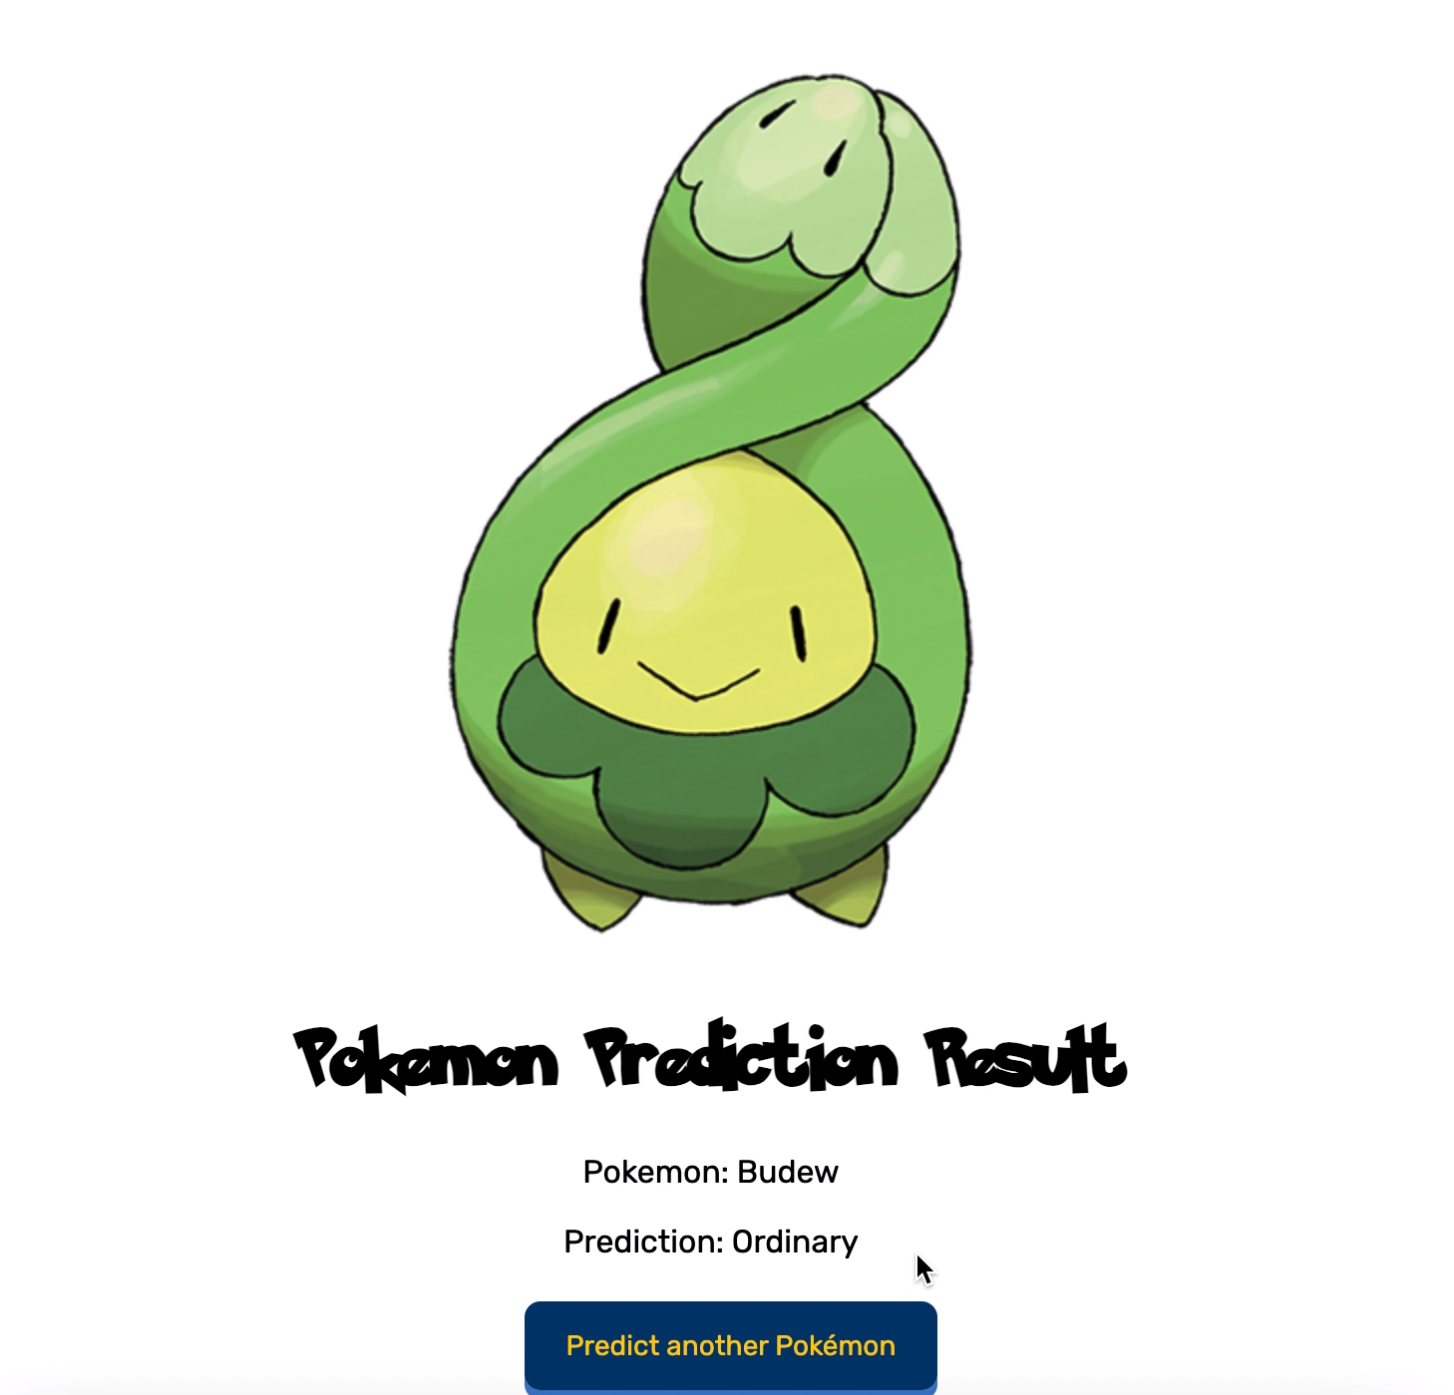
\includegraphics[width=1\linewidth]{website_output.png}
  \caption{Website Demonstration}
  \label{fig:your_photo}
\end{figure}

\section{Discussion}
The reported classification metrics demonstrate the performance of logistic regression and SVM models in classifying "legendary" and "ordinary" Pokémon based on various attributes. The metrics provide insights into different aspects of the models' performance, allowing us to gauge their strengths and areas for potential improvement.

Both models showcase promising performance in differentiating between "legendary" and "ordinary" Pokémon. However, the SVM model tends to outperform logistic regression across most evaluation metrics, indicating its efficacy in this classification task.

The inclusion of the "total stats" feature significantly influences the models' predictive capabilities, enabling better differentiation between the two Pokémon ranks. Yet, exploring the interactions among attributes and their impact on model predictions remains crucial for a comprehensive understanding of the models' behavior.

Further analysis, such as feature importance determination or model interpretability techniques, could provide deeper insights into the specific influence of features and algorithms on the models' classification performance.

\section{Conclusion}
By using a linear SVM model with the input features hp, attack, defense, special attack, special defense, speed, total stats, height and weight, we were able to predict the rank of Pokémon with a 93\% accuracy on our testing data. Although our model is quite accurate, we could have improved it by omitting features that we identified as not contributing to linearly separating the data in our exploratory data analysis. SVM machine learning will increase the magnitude of the weights for features that contribute more to creating an accurate decision boundary, so our model is still accurate even when including features that don't linearly separate the data. We can also improve the accuracy of our model by taking into account the categorical data we omitted initially, such as abilities. Although there are over 200 different Pokémon abilities, which would make our model quite computationally expensive, we can perform exploratory data analysis to determine which abilities are most common and omit the abilities with a sparse count. 

\begin{thebibliography}{00}
\bibitem{b1} Breddan, M. D. (2021, December 6). Gotta sort 'em all: Applying machine learning algorithms to Pokémon. Medium. https://medium.com/\%40mjdavis325/gotta-sort-em-all-applying-machine-learning-algorithms-to-pok\%C3\%A9mon-72ccce54abf7 
\bibitem{b2} Cyberpatcher, Hamza. “Data of 1017 Pokemons.” Kaggle, 25 Sept. 2023, www.kaggle.com/datasets/hamzacyberpatcher/data-of-1010-pokemons.
\end{thebibliography}
\end{document}